\documentclass{article}
\usepackage[a4paper, margin=.8in]{geometry}

\usepackage{amssymb}
\usepackage{varwidth}

\usepackage{siunitx}

\usepackage{fancyhdr}

\usepackage[utf8]{inputenc}
\usepackage{t1enc}
\def\magyarOptions{defaults=hu-min}
\usepackage[magyar]{babel}

\usepackage{graphicx}
\graphicspath{ {./} }

\usepackage{amsmath}

\usepackage{pdfpages}

\usepackage{pgf}

\usepackage{multicol}

\usepackage{bm}

\usepackage{tikz}
\usetikzlibrary {arrows.meta, decorations.markings}

\fancypagestyle{plain}{%
	\fancyhf{}%

	\fancyhead{}
	\fancyhead[L]{Vári Gergő}
	\fancyhead[C]{MQHJ0H}
	\fancyhead[R]{
\includegraphics[scale=.25]{signature}}
	\setlength{\headheight}{16.5pt}

	\fancyfoot{}
	\fancyfoot[C]{\thepage}
}

\pagestyle{plain}

\title{Statika 3. HF}
\author{Vári Gergő}
\date{\today}

\pgfmathsetmacro{\a}{1.2}
\pgfmathsetmacro{\b}{2}
\pgfmathsetmacro{\c}{1.5}

\pgfmathsetmacro{\Fa}{20}
\pgfmathsetmacro{\Fb}{32}
\pgfmathsetmacro{\Fc}{13}

\pgfmathsetmacro{\By}{- \Fb * ( \c / \b )}
\pgfmathsetmacro{\Cy}{\By}
\pgfmathsetmacro{\Ay}{\Fa - \Cy}
\pgfmathsetmacro{\Ax}{(-\Ay * 2* \a + \Fa * \a - \Fc * \c) / (\c)}
\pgfmathsetmacro{\Cx}{-\Ax - \Fc}
\pgfmathsetmacro{\Bx}{\Cx + \Fb}

\pgfmathsetmacro{\Nay}{\Ay}
\pgfmathsetmacro{\alfa}{atan(\c / \a)}
\pgfmathsetmacro{\Na}{\Nay / sin(\alfa)}
\pgfmathsetmacro{\Nax}{\Na * cos(\alfa)}
\pgfmathsetmacro{\Nb}{-\Ax - \Nax}
\pgfmathsetmacro{\Nc}{\Fa - \Nay}
\pgfmathsetmacro{\Nd}{\Fc}
\pgfmathsetmacro{\Nex}{\Nb - \Nd}
\pgfmathsetmacro{\Ney}{-\Nc}
\pgfmathsetmacro{\Ne}{sqrt((\Nex^2 + \Ney^2))}
\pgfmathsetmacro{\Nf}{\Nax}
\pgfmathsetmacro{\Ng}{0}
\pgfmathsetmacro{\Nh}{\Bx}
\pgfmathsetmacro{\Beta}{atan(\b / \c)}
\pgfmathsetmacro{\Nix}{-\Fb}
\pgfmathsetmacro{\Ni}{\Nix / sin(\Beta)}
\pgfmathsetmacro{\Niy}{\Ni * cos(\Beta)}
\pgfmathsetmacro{\Nj}{-\By}

\newcommand{\pnum}[1]{%
	\pgfmathprintnumber[fixed]{#1}
}

\begin{document}


\pgfmathsetmacro{\unitm}{2.5}
\pgfmathsetmacro{\shownm}{1}
\pgfmathsetmacro{\unitkn}{1/10}
\pgfmathsetmacro{\shownkn}{10}

\pgfmathsetmacro{\as}{\a * \unitm}
\pgfmathsetmacro{\bs}{\b * \unitm}
\pgfmathsetmacro{\cs}{\c * \unitm}

\pgfmathsetmacro{\Fas}{\Fa * \unitkn}
\pgfmathsetmacro{\Fbs}{\Fb * \unitkn}
\pgfmathsetmacro{\Fcs}{\Fc * \unitkn}

\newcommand{\struccoordsys}{%
	\draw[thick,->] (0,0) -- ++(1,0) node[anchor=north west] {x};
	\draw[thick,->] (0,0) -- ++(0,1) node[anchor=south east] {y};
}
\newcommand{\strucbend}{%
	\draw[->] (2,0) to [bend right] node[midway, above] {+} ++(1,0);
}

\newcommand{\strucguide}{%
	\begin{tikzpicture}
		\struccoordsys
		\strucbend
		
		\draw[thick,arrows = {Bracket-Bracket}] (0,-1) -- ++(\unitm * \shownm,0) node[midway, below] {\shownm [\si{m}]};
		\draw[thick,arrows = {Bracket-Bracket}] (0,-2) -- ++(\unitkn * \shownkn,0) node[midway, below] {\shownkn [\si{kN}]};
	\end{tikzpicture}
}

\newcommand{\strucframe}{%
	\coordinate (A) at (0, \cs);
	\coordinate (B) at (2*\as + \bs, 0);
	\coordinate (C) at (2*\as, 0);
	\coordinate (D) at (\as, \cs);
	\coordinate (E) at (\as, 0);
	\coordinate (F) at (2*\as, \cs);
	\coordinate (G) at (2*\as + \bs, \cs);

	\draw[line width = 0.1mm] (-1,0) -- (E);
	\draw[line width = 0.1mm] (-1,\cs) -- (G);
	\draw[line width = 0.1mm] (A)++(0,2) -- ++(0,-\cs-4);
	\draw[line width = 0.1mm] (D)++(0,2) -- ++(0,-\cs-4);
	\draw[line width = 0.1mm] (F)++(0,2) -- ++(0,-\cs-4);
	\draw[line width = 0.1mm] (G)++(0,2) -- ++(0,-\cs-4);

	\draw[line width = 0.2mm, arrows = {Latex-Latex}] (-1,0) -- ++(0,\cs) node[midway, left] {c};
	\draw[line width = 0.2mm, arrows = {Latex-Latex}] (0,-1) -- ++(\as,0) node[midway, below] {a};
	\draw[line width = 0.2mm, arrows = {Latex-Latex}] (\as,-1) -- ++(\as,0) node[midway, below] {a};
	\draw[line width = 0.2mm, arrows = {Latex-Latex}] (2*\as,-1) -- ++(\bs,0) node[midway, below] {b};
	
	\pgfmathsetmacro{\framewidth}{.7mm}
	\draw[line width = \framewidth, arrows = {-}] (A) -- (E) node[midway, anchor=north east] {1};
	\draw[line width = \framewidth, arrows = {-}] (A) -- (D) node[midway, above] {2};
	\draw[line width = \framewidth, arrows = {-}] (D) -- (E) node[midway, left] {3};
	\draw[line width = \framewidth, arrows = {-}] (D) -- (F) node[midway, above] {4};
	\draw[line width = \framewidth, arrows = {-}] (D) -- (C) node[midway, anchor=south west] {5};
	\draw[line width = \framewidth, arrows = {-}] (E) -- (C) node[midway, below] {6};
	\draw[line width = \framewidth, arrows = {-}] (F) -- (C) node[midway, right] {7};
	\draw[line width = \framewidth, arrows = {-}] (C) -- (B) node[midway, below] {8};
	\draw[line width = \framewidth, arrows = {-}] (C) -- (G) node[midway, anchor=north west] {9};
	\draw[line width = \framewidth, arrows = {-}] (B) -- (G) node[midway, right] {10};

	\foreach \point/\name in {A, D, F, G} {
		\fill[white] (\point) circle[radius=2.5pt];
		\draw[thick] (\point) circle[radius=2pt] node[anchor=south west] {\name};
	}
	\foreach \point/\name in {C} {
		\fill[white] (\point) circle[radius=2.5pt];
		\draw[thick] (\point) circle[radius=2pt] node[anchor=north west] {\name};
	}
	\foreach \point/\name in {B, E} {
		\fill[white] (\point) circle[radius=2.5pt];
		\draw[thick] (\point) circle[radius=2pt] node[anchor=south west] {\name};
	}
}

\newcommand{\strucforces}{%
	\draw[line width = .8mm, arrows = {-Stealth}, blue] (F) -- ++(\Fcs, 0) node[midway, above] {$F_3$};
	\draw[line width = .8mm, arrows = {-Stealth}, blue] (E) -- ++(0, -\Fas) node[right] {$F_1$};
	\draw[line width = .8mm, arrows = {Stealth-}, blue] (G) -- ++(\Fbs, 0) node[midway, above] {$F_2$};
}

\newcommand{\strucrestraints}{%
	\pgfmathsetmacro{\restrainsize}{.4}
	\draw[line width = .4mm, green] (A) -- ++(-\restrainsize, \restrainsize) -- ++(0, -\restrainsize * 2) -- cycle;
	\draw[line width = .4mm, green] (A)++(-\restrainsize, \restrainsize*1.5) -- ++(0, -\restrainsize * 2 * 1.5);
	\draw[line width = .4mm, green] (A)++(-\restrainsize, 0.4) -- ++(-0.2, .2);
	\draw[line width = .4mm, green] (A)++(-\restrainsize, 0.2) -- ++(-0.2, .2);
	\draw[line width = .4mm, green] (A)++(-\restrainsize, 0) -- ++(-0.2, .2);
	\draw[line width = .4mm, green] (A)++(-\restrainsize, -0.2) -- ++(-0.2, .2);
	\draw[line width = .4mm, green] (A)++(-\restrainsize, -0.4) -- ++(-0.2, .2);
	\draw[line width = .4mm, green] (A)++(-\restrainsize, -0.6) -- ++(-0.2, .2);

	\draw[line width = .4mm, green] (B) -- ++(-\restrainsize, -\restrainsize) -- ++(\restrainsize * 2, 0) -- cycle;
	\draw[line width = .4mm, green] (B)++(-\restrainsize*1.5, -\restrainsize) -- ++(\restrainsize * 2 * 1.5, 0);
	\draw[line width = .4mm, green] (B)++(0.6, -\restrainsize) -- ++(-0.2, -.2);
	\draw[line width = .4mm, green] (B)++(0.4, -\restrainsize) -- ++(-0.2, -.2);
	\draw[line width = .4mm, green] (B)++(0.2, -\restrainsize) -- ++(-0.2, -.2);
	\draw[line width = .4mm, green] (B)++(0, -\restrainsize) -- ++(-0.2, -.2);
	\draw[line width = .4mm, green] (B)++(-0.2, -\restrainsize) -- ++(-0.2, -.2);
	\draw[line width = .4mm, green] (B)++(-0.4, -\restrainsize) -- ++(-0.2, -.2);
}


% 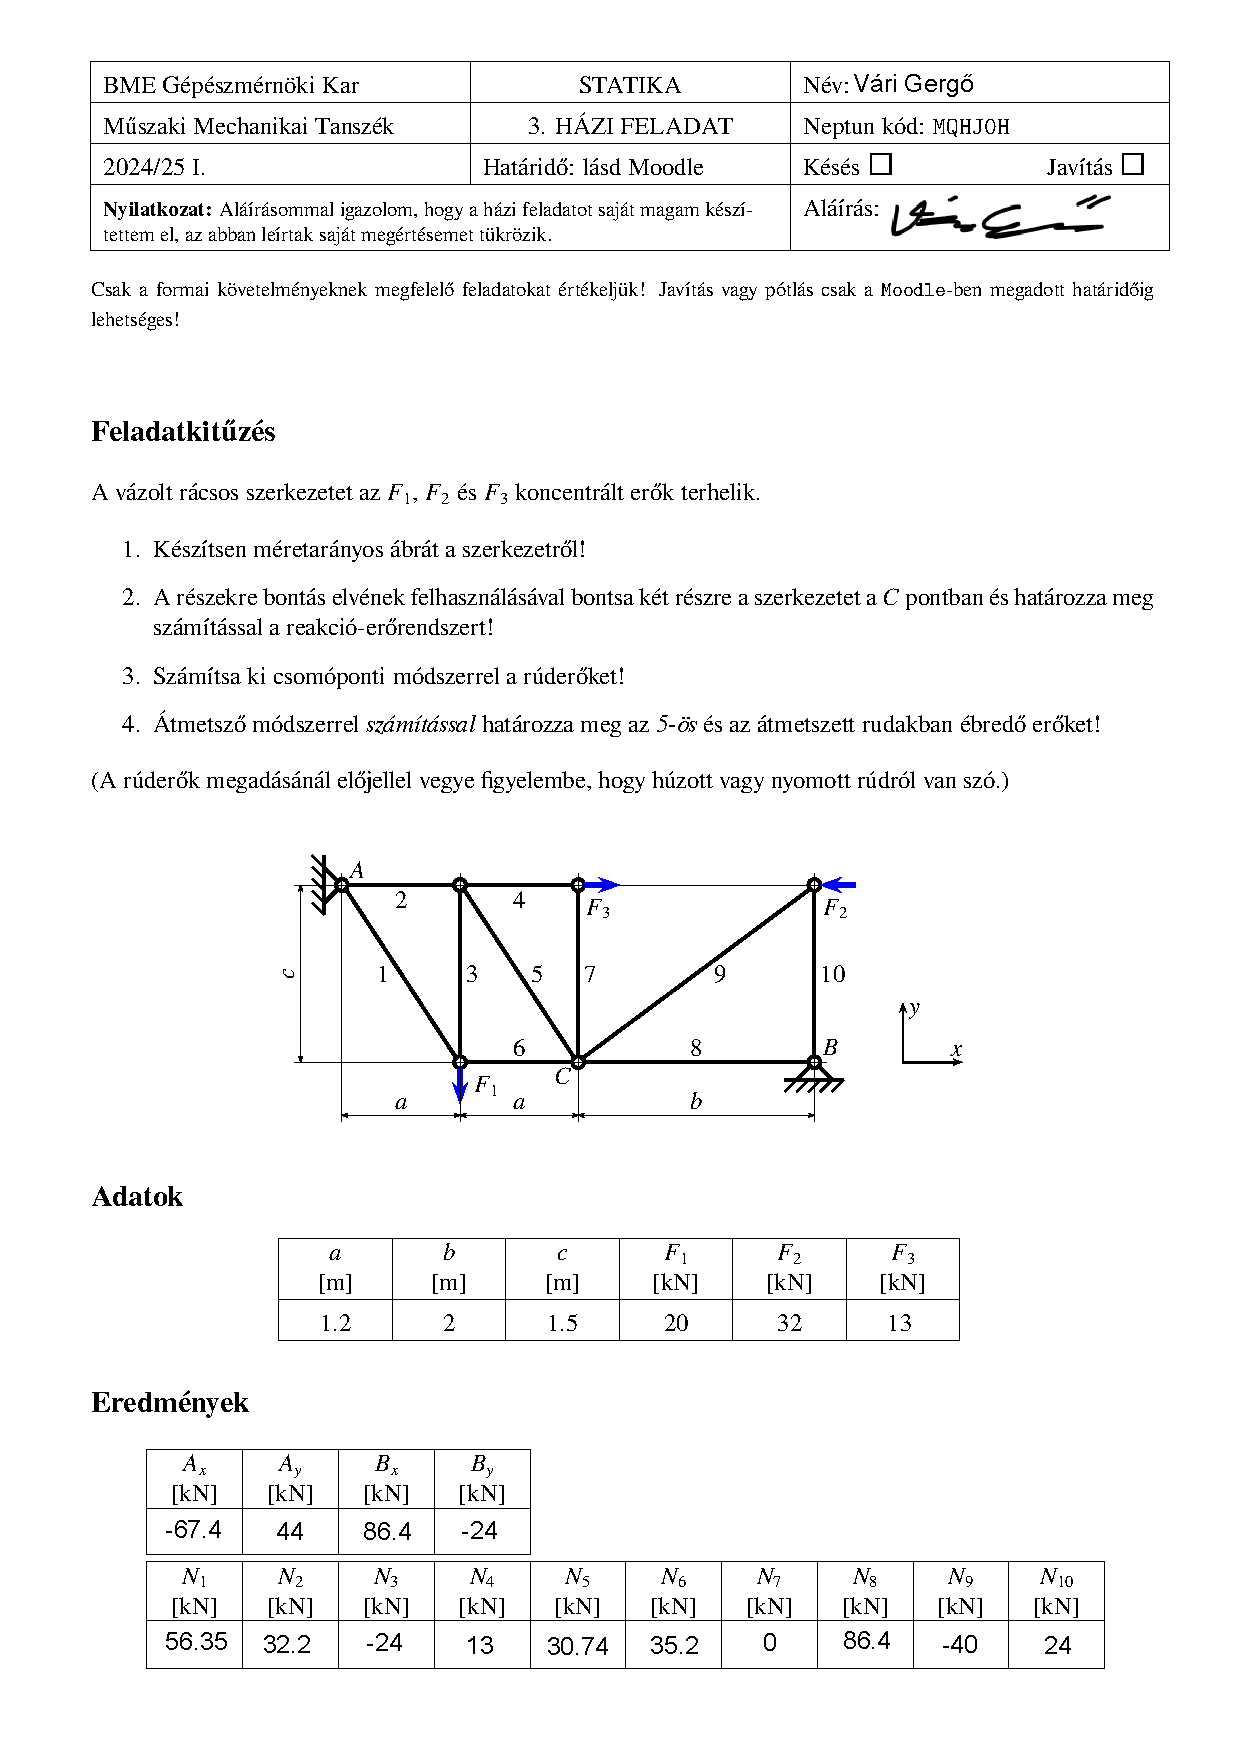
\includepdf[pages={1}]{sthf3-final.pdf} %

\maketitle


\section{Méretarányos ábra}

\pgfmathsetmacro{\unitm}{2.5}
\pgfmathsetmacro{\shownm}{1}
\pgfmathsetmacro{\unitkn}{1/10}
\pgfmathsetmacro{\shownkn}{10}

\pgfmathsetmacro{\as}{\a * \unitm}
\pgfmathsetmacro{\bs}{\b * \unitm}
\pgfmathsetmacro{\cs}{\c * \unitm}

\pgfmathsetmacro{\Fas}{\Fa * \unitkn}
\pgfmathsetmacro{\Fbs}{\Fb * \unitkn}
\pgfmathsetmacro{\Fcs}{\Fc * \unitkn}

\newcommand{\strucguide}{%
	\begin{tikzpicture}
		\draw[thick,->] (0,0) -- ++(1,0) node[anchor=north west] {x};
		\draw[thick,->] (0,0) -- ++(0,1) node[anchor=south east] {y};
		
		\draw[->] (2,0) to [bend right] node[midway, above] {+} ++(1,0);
		
		\draw[thick,arrows = {Bracket-Bracket}] (0,-1) -- ++(\unitm * \shownm,0) node[midway, below] {\shownm [\si{m}]};
		\draw[thick,arrows = {Bracket-Bracket}] (0,-2) -- ++(\unitkn * \shownkn,0) node[midway, below] {\shownkn [\si{kN}]};
	\end{tikzpicture}
}

\newcommand{\strucframe}{%
	\coordinate (A) at (0, \cs);
	\coordinate (B) at (2*\as + \bs, 0);
	\coordinate (C) at (2*\as, 0);
	\coordinate (D) at (\as, \cs);
	\coordinate (E) at (\as, 0);
	\coordinate (F) at (2*\as, \cs);
	\coordinate (G) at (2*\as + \bs, \cs);

	\draw[line width = 0.1mm] (-1,0) -- (E);
	\draw[line width = 0.1mm] (-1,\cs) -- (G);
	\draw[line width = 0.1mm] (A) -- (0,-2);

	\draw[line width = 0.2mm, arrows = {Bracket-Bracket}] (-1,0) -- ++(0,\cs) node[midway, left] {c};
	\draw[line width = 0.2mm, arrows = {Bracket-Bracket}] (0,-1) -- ++(\as,0) node[midway, below] {a};
	\draw[line width = 0.2mm, arrows = {Bracket-Bracket}] (\as,-1) -- ++(\as,0) node[midway, below] {a};
	\draw[line width = 0.2mm, arrows = {Bracket-Bracket}] (2*\as,-1) -- ++(\bs,0) node[midway, below] {b};

	\draw[line width = .5mm, arrows = {-}] (A) -- (E) node[midway, left] {1};
	\draw[line width = .5mm, arrows = {-}] (A) -- (D) node[midway, above] {2};
	\draw[line width = .5mm, arrows = {-}] (D) -- (E) node[midway, left] {3};
	\draw[line width = .5mm, arrows = {-}] (D) -- (F) node[midway, above] {4};
	\draw[line width = .5mm, arrows = {-}] (D) -- (C) node[midway, anchor=south west] {5};
	\draw[line width = .5mm, arrows = {-}] (E) -- (C) node[midway, below] {6};
	\draw[line width = .5mm, arrows = {-}] (F) -- (C) node[midway, right] {7};
	\draw[line width = .5mm, arrows = {-}] (C) -- (B) node[midway, below] {8};
	\draw[line width = .5mm, arrows = {-}] (C) -- (G) node[midway, anchor=north west] {9};
	\draw[line width = .5mm, arrows = {-}] (B) -- (G) node[midway, right] {10};

	\foreach \point/\name in {A, D, F, G} {
		\fill[white] (\point) circle[radius=2.5pt];
		\draw[thick] (\point) circle[radius=2pt] node[anchor=south] {\name};
	}
	\foreach \point/\name in {C} {
		\fill[white] (\point) circle[radius=2.5pt];
		\draw[thick] (\point) circle[radius=2pt] node[anchor=north] {\name};
	}
	\foreach \point/\name in {B, E} {
		\fill[white] (\point) circle[radius=2.5pt];
		\draw[thick] (\point) circle[radius=2pt] node[anchor=south west] {\name};
	}
}

\newcommand{\strucforces}{%
	\draw[line width = .8mm, arrows = {-Stealth}, blue] (F) -- ++(\Fcs, 0) node[midway, above] {$F_3$};
	\draw[line width = .8mm, arrows = {-Stealth}, blue] (E) -- ++(0, -\Fas) node[right] {$F_1$};
	\draw[line width = .8mm, arrows = {Stealth-}, blue] (G) -- ++(\Fbs, 0) node[midway, above] {$F_2$};
}

\newcommand{\strucrestraints}{%
	\pgfmathsetmacro{\restrainsize}{.4}
	\draw[line width = .4mm, green] (A) -- ++(-\restrainsize, \restrainsize) -- ++(0, -\restrainsize * 2) -- cycle;
	\draw[line width = .4mm, green] (A)++(-\restrainsize, \restrainsize*1.5) -- ++(0, -\restrainsize * 2 * 1.5);
	\draw[line width = .4mm, green] (A)++(-\restrainsize, 0.4) -- ++(-0.2, .2);
	\draw[line width = .4mm, green] (A)++(-\restrainsize, 0.2) -- ++(-0.2, .2);
	\draw[line width = .4mm, green] (A)++(-\restrainsize, 0) -- ++(-0.2, .2);
	\draw[line width = .4mm, green] (A)++(-\restrainsize, -0.2) -- ++(-0.2, .2);
	\draw[line width = .4mm, green] (A)++(-\restrainsize, -0.4) -- ++(-0.2, .2);
	\draw[line width = .4mm, green] (A)++(-\restrainsize, -0.6) -- ++(-0.2, .2);

	\draw[line width = .4mm, green] (B) -- ++(-\restrainsize, -\restrainsize) -- ++(\restrainsize * 2, 0) -- cycle;
	\draw[line width = .4mm, green] (B)++(-\restrainsize*1.5, -\restrainsize) -- ++(\restrainsize * 2 * 1.5, 0);
	\draw[line width = .4mm, green] (B)++(0.6, -\restrainsize) -- ++(-0.2, -.2);
	\draw[line width = .4mm, green] (B)++(0.4, -\restrainsize) -- ++(-0.2, -.2);
	\draw[line width = .4mm, green] (B)++(0.2, -\restrainsize) -- ++(-0.2, -.2);
	\draw[line width = .4mm, green] (B)++(0, -\restrainsize) -- ++(-0.2, -.2);
	\draw[line width = .4mm, green] (B)++(-0.2, -\restrainsize) -- ++(-0.2, -.2);
	\draw[line width = .4mm, green] (B)++(-0.4, -\restrainsize) -- ++(-0.2, -.2);
}

\begin{center}
	\strucguide
	\begin{tikzpicture}
		\strucframe
		\strucforces
		\strucrestraints
	\end{tikzpicture}
\end{center}


\section{Részekre bontás elve}

\subsection{Szabadtest-ábra (SZTÁ)}
\begin{center}
	\begin{tikzpicture}
		\struccoordsys
		\strucbend
	\end{tikzpicture}
	\begin{tikzpicture}
		\strucframe
		\strucforces
		\strucrestrainforces
		\foreach \point in {C} {
			\fill[thick, orange] (\point) circle[radius=4pt];
		}
	\end{tikzpicture}
\end{center}

\subsection{Részek vizsgálata}
\begin{multicols}{2}

\subsubsection{}
\begin{center}
	\begin{tikzpicture}
		\strucframepartone
		\strucforcespartone
		\strucrestrainforcespartone
		\foreach \point in {C} {
			\fill[thick, orange] (\point) circle[radius=4pt];
		}
		\struccutforcespartone
	\end{tikzpicture}
\end{center}
\begin{align*}
	&\sum{\vec{F}_x} := 0 = A_x + F_3 + C_x \\
	&\sum{\vec{F}_y} := 0 = A_y - F_1 + C_y \\
	&\sum{\vec{M}_C} := 0 = -A_x \times c - A_y \times 2a + F_1 \times a -F_3 \times c
\end{align*}

\begin{align*}
	&A_y = F_1 - C_y &= \pgfmathprintnumber[fixed]{\Ay} [\si{kN}] \\
	&A_x = \frac{-A_y \times 2a+F_1 \times a - F_3 \times c}{c} &= \pgfmathprintnumber[fixed]{\Ax} [\si{kN}] \\
	&C_x = -A_x - F_3 &= \pgfmathprintnumber[fixed]{\Cx} [\si{kN}]
\end{align*}

\subsubsection{}
\begin{center}
	\begin{tikzpicture}
		\strucframeparttwo
		\strucforcesparttwo
		\strucrestrainforcesparttwo
		\foreach \point in {C} {
			\fill[thick, orange] (\point) circle[radius=4pt];
		}
		\struccutforcesparttwo
	\end{tikzpicture}
\end{center}
\begin{align*}
	&\sum{\vec{F}_x} := 0 = B_x - F_2 - C_x \\
	&\sum{\vec{F}_y} := 0 = B_y - C_y \\
	&\sum{\vec{M}_C} := 0 = F_2 \times c + B_y \times b
\end{align*}

\begin{align*}
	&B_y = -F_2 \frac{c}{b} &= \pgfmathprintnumber[fixed]{\By} [\si{kN}] \\
	&C_y = B_y &= \pgfmathprintnumber[fixed]{\Cy} [\si{kN}] \\
	&B_x = C_x + F_2 &= \pgfmathprintnumber[fixed]{\Bx} [\si{kN}]
\end{align*}

\end{multicols}

\begin{center}
	\fbox{
	    $
		\begin{aligned}
		    A &= \begin{bmatrix}
			    \pgfmathprintnumber[fixed]{\Ax} \\
			    \pgfmathprintnumber[fixed]{\Ay}
		    \end{bmatrix} &[\si{kN}]\\
		    B &= \begin{bmatrix}
			    \pgfmathprintnumber[fixed]{\Bx} \\
			    \pgfmathprintnumber[fixed]{\By}
		    \end{bmatrix} &[\si{kN}]
		\end{aligned}
	    $
	}
\end{center}


\newcommand{\sepline}{%
	\begin{center}
	    \rule{\linewidth}{0.4pt}
	\end{center}
}

\section{Csomóponti módszer}

% A
\begin{minipage}{0.4\textwidth}
	\centering
	\begin{tikzpicture}
		\draw circle (1) node[midway, font=\huge] {A};
		\draw[line width = .8mm, arrows = {-Stealth}, cyan] (1, 0) -- ++(2, 0) node[midway, above] {$N_2$};
		\draw[line width = .8mm, arrows = {-Stealth}, blue] (-3, 0) -- ++(2, 0) node[midway, above] {$A_x$};
		\draw[line width = .8mm, arrows = {-Stealth}, blue] (0, -3) -- ++(0, 2) node[midway, left] {$A_y$};
		\draw[line width = .8mm, arrows = {-Stealth}, cyan] (-\alfa:1) -- ++(-\alfa:2) node[midway, left] {$N_1$};
		\draw[black] (2, 0) arc[start angle=0, end angle=-\alfa, radius=2] node[midway, anchor=south east, font=\huge] {$\alpha$};

	\end{tikzpicture}
\end{minipage}
\begin{minipage}{0.5\textwidth}
	\begin{align*}
		&\sum{\vec{F}_x} := 0 = A_x + N_2 + {N_1}_x\\
		&\sum{\vec{F}_y} := 0 = A_y - {N_1}_y
	\end{align*}
	\begin{center}
		$\tan \alpha = \frac{c}{a} \Rightarrow \alpha = \pnum{\alfa}$\textdegree
	\end{center}
	\begin{align*}
		&{N_1}_y = A_y = &\pnum{\Nay} [\si{kN}] \\
		&\mathbf{N_1} = \frac{{N_1}_y}{\sin \alpha} = &\mathbf{\pnum{\Na}} [\si{kN}] \\
		&{N_1}_x = N_1 \times \cos \alpha = &\pnum{\Nax} [\si{kN}]
	\end{align*}
\end{minipage}


\sepline

% B
\begin{minipage}{0.4\textwidth}
	\centering
	\begin{tikzpicture}
		\draw circle (1) node[midway, font=\huge] {B};
		\draw[line width = .8mm, arrows = {-Stealth}, cyan] (-1, 0) -- ++(-2, 0) node[midway, above] {$N_8$};
		\draw[line width = .8mm, arrows = {-Stealth}, blue] (1, 0) -- ++(2, 0) node[midway, above] {$B_x$};
		\draw[line width = .8mm, arrows = {-Stealth}, blue] (0, -3) -- ++(0, 2) node[midway, left] {$B_y$};
		\draw[line width = .8mm, arrows = {-Stealth}, cyan] (0, 1) -- ++(0, 2) node[midway, left] {$N_{10}$};

	\end{tikzpicture}
\end{minipage}
\begin{minipage}{0.5\textwidth}
	\begin{align*}
		&\sum{\vec{F}_x} := 0 = B_x - N_8 \\
		&\sum{\vec{F}_y} := 0 = B_y + N_{10}
	\end{align*}
	\begin{align*}
		\mathbf{N_8} &= B_x = &\mathbf{\pnum{\Nh}} [\si{kN}] \\
		\mathbf{N_{10}} &= -B_y = &\mathbf{\pnum{\Nj}} [\si{kN}]
	\end{align*}
\end{minipage}

\sepline

% C
\begin{minipage}{0.4\textwidth}
	\centering
	\begin{tikzpicture}
		\draw circle (1) node[midway, font=\huge] {C};
		\draw[line width = .8mm, arrows = {-Stealth}, cyan] (180-\alfa:1) -- ++(180-\alfa:2) node[midway, right] {$N_5$};
		\draw[black] (-2, 0) arc[start angle=180, end angle=180-\alfa, radius=2] node[midway, anchor=north west, font=\huge] {$\alpha$};
		\draw[line width = .8mm, arrows = {-Stealth}, cyan] (-1, 0) -- ++(-2, 0) node[midway, below] {$N_6$};
		\draw[line width = .8mm, arrows = {-Stealth}, cyan] (0, 1) -- ++(0, 2) node[midway, left] {$N_7$};
		\draw[line width = .8mm, arrows = {-Stealth}, cyan] (1, 0) -- ++(2, 0) node[midway, below] {$N_8$};
		\draw[line width = .8mm, arrows = {-Stealth}, cyan] (90-\Beta:1) -- ++(90-\Beta:2) node[midway, anchor=south east] {$N_9$};
		\draw[black] (2.5, 0) arc[start angle=0, end angle=90-\Beta, radius=2.5] node[midway, anchor=north east] {$\ang{90}-\beta$};
	\end{tikzpicture}
\end{minipage}
\begin{minipage}{0.5\textwidth}
	\begin{align*}
		&\sum{\vec{F}_x} := 0 = N_8 - N_6 + {N_9}_x - {N_5}_x \\
		&\sum{\vec{F}_y} := 0 = N_7 + {N_5}_y + {N_9}_y 
	\end{align*}
	\begin{align*}
		&\mathbf{N_6} = N_8 + {N_9}_x - {N_5}_x = &\mathbf{\pnum{\Nf}} [\si{kN}] \\
		&\mathbf{N_7} = -{N_5}_y - {N_9}_y = &\mathbf{\pnum{\Ng}} [\si{kN}]
	\end{align*}
\end{minipage}

\sepline

% D
\begin{minipage}{0.4\textwidth}
	\centering
	\begin{tikzpicture}
		\draw circle (1) node[midway, font=\huge] {D};
		\draw[line width = .8mm, arrows = {-Stealth}, cyan] (1, 0) -- ++(2, 0) node[midway, above] {$N_4$};
		\draw[line width = .8mm, arrows = {-Stealth}, cyan] (-1, 0) -- ++(-2, 0) node[midway, above] {$N_2$};
		\draw[line width = .8mm, arrows = {-Stealth}, cyan] (0, -1) -- ++(0, -2) node[midway, left] {$N_3$};
		\draw[line width = .8mm, arrows = {-Stealth}, cyan] (-\alfa:1) -- ++(-\alfa:2) node[midway, left] {$N_5$};
		\draw[black] (2, 0) arc[start angle=0, end angle=-\alfa, radius=2] node[midway, anchor=south east, font=\huge] {$\alpha$};

	\end{tikzpicture}
\end{minipage}
\begin{minipage}{0.5\textwidth}
	\begin{align*}
		&\sum{\vec{F}_x} := 0 = N_4 - N_2 + {N_5}_x \\
		&\sum{\vec{F}_y} := 0 = -N_3 - {N_5}_y 
	\end{align*}
	\begin{align*}
		{N_5}_x &= N_2 - N_4 = &\mathbf{\pnum{\Nex}} [\si{kN}] \\
		{N_5}_y &= -N_3 = &\mathbf{\pnum{\Ney}} [\si{kN}] \\
		\mathbf{N_5} &= \sqrt{{{N_5}_x}^2 + {{N_5}_y}^2} = &\mathbf{\pnum{\Ne}} [\si{kN}] \\
	\end{align*}
\end{minipage}

\sepline

% E
\begin{minipage}{0.4\textwidth}
	\centering
	\begin{tikzpicture}
		\draw circle (1) node[midway, font=\huge] {E};
		\draw[line width = .8mm, arrows = {-Stealth}, cyan] (180-\alfa:1) -- ++(180-\alfa:2) node[midway, right] {$N_1$};
		\draw[black] (-2, 0) arc[start angle=180, end angle=180-\alfa, radius=2] node[midway, anchor=north west, font=\huge] {$\alpha$};
		\draw (-1, 0) -- ++(-2, 0);
		\draw[line width = .8mm, arrows = {-Stealth}, cyan] (0, 1) -- ++(0, 2) node[midway, right] {$N_3$};
		\draw[line width = .8mm, arrows = {-Stealth}, cyan] (1, 0) -- ++(2, 0) node[midway, below] {$N_8$};
		\draw[line width = .8mm, arrows = {-Stealth}, blue] (0, -1) -- ++(0, -2) node[midway, left] {$F_1$};
	\end{tikzpicture}
\end{minipage}
\begin{minipage}{0.5\textwidth}
	\begin{align*}
		&\sum{\vec{F}_x} := 0 = N_6 - {N_1}_x \\
		&\sum{\vec{F}_y} := 0 = N_3 - F_1 + {N_1}_y
	\end{align*}
	\begin{align*}
		&N_6 = {N_1}_x = &\pnum{\Nf} &[\si{kN}] \checkmark \\
		&\mathbf{N_3} = F_1 - {N_1}_y = &\mathbf{\pnum{\Nc}} &[\si{kN}] \\
	\end{align*}
\end{minipage}

\sepline

% F
\begin{minipage}{0.4\textwidth}
	\centering
	\begin{tikzpicture}
		\draw circle (1) node[midway, font=\huge] {F};
		\draw[line width = .8mm, arrows = {-Stealth}, cyan] (-1, 0) -- ++(-2, 0) node[midway, below] {$N_4$};
		\draw[line width = .8mm, arrows = {-Stealth}, blue] (1, 0) -- ++(2, 0) node[midway, below] {$F_3$};
		\draw[line width = .8mm, arrows = {-Stealth}, cyan] (0, -1) -- ++(0, -2) node[midway, left] {$N_7$};
	\end{tikzpicture}
\end{minipage}
\begin{minipage}{0.5\textwidth}
	\begin{align*}
		&\sum{\vec{F}_x} := 0 = F_3 - N_4 \\
		&\sum{\vec{F}_y} := 0 = -N_7
	\end{align*}
	\begin{align*}
		&\mathbf{N_4} = F_3 = &\mathbf{\pnum{\Nd}} &[\si{kN}] \\
		&N_7 = &\pnum{\Ng} &[\si{kN}] \checkmark \\
	\end{align*}
\end{minipage}

\sepline

% G
\begin{minipage}{0.4\textwidth}
	\centering
	\begin{tikzpicture}
		\draw circle (1) node[midway, font=\huge] {G};
		\draw[line width = .8mm, arrows = {-Stealth}, cyan] (180+\Beta:1) -- ++(180+\Beta:2) node[midway, anchor=south east] {$N_9$};
		\draw (180+\Beta:2) arc[start angle=180+\Beta, end angle=270, radius=2] node[midway, above, font=\LARGE] {$\beta$};
		\draw[line width = .8mm, arrows = {-Stealth}, cyan] (0, -1) -- ++(0, -2) node[midway, right] {$N_{10}$};
		\draw (-1, 0) -- ++(-2, 0);
		\draw[line width = .8mm, arrows = {-Stealth}, blue] (3, 0) -- ++(-2, 0) node[midway, below] {$F_2$};
	\end{tikzpicture}
\end{minipage}
\begin{minipage}{0.5\textwidth}
	\begin{align*}
		&\sum{\vec{F}_x} := 0 = -F_2 - {N_9}_x \\
		&\sum{\vec{F}_y} := 0 = -N_{10} - {N_9}_y 
	\end{align*}
	\begin{center}
		$\tan \beta = \frac{b}{c} \Rightarrow \beta = \pnum{\Beta}$\textdegree
	\end{center}
	\begin{align*}
		{N_9}_x &= -F_2 = &\mathbf{\pnum{\Nix}} [\si{kN}] \\
		\mathbf{N_9} &= \frac{{N_9}_x}{\sin\beta} = &\mathbf{\pnum{\Ni}} [\si{kN}] \\
		{N_9}_y &= N_9 \times \cos\beta = &\mathbf{\pnum{\Niy}} [\si{kN}] \\
		\mathbf{N_{10}} &= -{N_9}_y = &\mathbf{\pnum{\Nj}} [\si{kN}]
	\end{align*}
\end{minipage}


\section{Átmetsző módszer}

\subsection{SZTÁ}
\begin{center}
	\begin{tikzpicture}
		\struccoordsys
		\strucbend
	\end{tikzpicture}
	\begin{tikzpicture}
		\strucframe
		\strucforces
		\strucrestrainforces
		\draw[loosely dashed, orange, line width=.8mm] ($ (D) !0.5! (F) $)+(-.5,2) -- ($ ($ (E) !0.5! (C) $) + (-.5, -2)$);
	\end{tikzpicture}
\end{center}

\subsection{Megmaradt rúderők}
\begin{center}
	\begin{tikzpicture}
		\coordinate (A) at (0, \cs);
		\coordinate (D) at (\as, \cs);
		\coordinate (E) at (\as, 0);

		\draw[line width = 0.1mm] (A)+(-1,0) -- (A);
		\draw[line width = 0.1mm] (-1,0) -- (E);
		\draw[line width = 0.1mm] (A)++(0,2) -- ++(0,-\cs-4);
		\draw[line width = 0.1mm] (D)++(0,2) -- ++(0,-\cs-4);

		\draw[line width = 0.2mm, arrows = {Latex-Latex}] (-1,0) -- ++(0,\cs) node[midway, left] {c};
		\draw[line width = 0.2mm, arrows = {Latex-Latex}] (0,-1) -- ++(\as,0) node[midway, below] {a};

		\pgfmathsetmacro{\framewidth}{.7mm}
		\draw[line width = \framewidth, arrows = {-}] (A) -- (E) node[midway, anchor=north east] {1};
		\draw[line width = \framewidth, arrows = {-}] (A) -- (D) node[midway, above] {2};
		\draw[line width = \framewidth, arrows = {-}] (D) -- (E) node[midway, left] {3};

		\foreach \point/\name in {A, D} {
			\fill[white] (\point) circle[radius=2.5pt];
			\draw[thick] (\point) circle[radius=2pt] node[anchor=south west] {\name};
		}
		\foreach \point/\name in {E} {
			\fill[white] (\point) circle[radius=2.5pt];
			\draw[thick] (\point) circle[radius=2pt] node[anchor=south west] {\name};
		}

		\draw[line width = .8mm, arrows = {-Stealth}, blue] (E) -- ++(0, -\Fasp) node[right] {$F_1$};
		\draw[line width = .8mm, arrows = {-Stealth}, cyan] (D) -- ++(3, 0) node[midway, above] {$N_4$};

		\draw[line width = .8mm, arrows = {-Stealth}, cyan] (D) -- ++(-\alfa:3) node[midway, left] {$N_5$};
		\draw[black] (D) ++(2,0) arc[start angle=0, end angle=-\alfa, radius=2] node[midway, anchor=south east, font=\huge] {$\alpha$};

		\draw[line width = .8mm, arrows = {-Stealth}, cyan] (E) -- ++(3, 0) node[midway, above] {$N_6$};

	\draw[line width = .8mm, arrows = {-Stealth}, green] (A)++(-2, 0) -- (A) node[midway, above] {$A_x$};
	\draw[line width = .8mm, arrows = {-Stealth}, green] (A)++(0, -2) -- (A) node[midway, left] {$A_y$};
	\end{tikzpicture}
\end{center}

\begin{align*}
	&\sum{\vec{F}_x} := 0 = A_x + N_4 + {N_5}_x + N_6 \\
	&\sum{\vec{F}_y} := 0 = A_y - {N_5}_y - F_1 \\
	&\sum{\vec{M}_D} := 0 = A_y \times a + N_6 \times c \\
\end{align*}

\begin{align*}
	{N_5}_y &= A_y - F_2 = \pnum{\Ney} \checkmark \\
	\mathbf{N_5} &= \frac{{N_5}_y}{\sin\alpha} = \mathbf{\pnum{\Ne}} \checkmark \\
\end{align*}

\begin{align*}
	{N_5}_x &= N_5 \times \cos\alpha = \pnum{\Nex} \checkmark \\
	N_4 &= -A_x - {N_5}_x - N_6 = \pnum{\Nd} \checkmark \\
	N_6 &= \frac{A_y \times a}{c} = \pnum{\Nf} \checkmark \\
\end{align*}


\end{document}
